\section{Results}
\label{sec:results}

\begin{Remark}
Every numeric value in this section is generated by the analysis pipeline into
\texttt{numbers.tex}. Until the campaign has been executed the macros expand to
visible markers, so an unfilled value cannot reach a submitted document.
\end{Remark}

\subsection{Bi-factor calibration}

Fitting Algorithm~\ref{alg:calibration} to the factorial grid of X1 and X3
gives a consensus exponent $\bhat=\resBeta$ (standard error $\resBetaSE$) and a
client exponent $\ghat=\resGamma$ (standard error $\resGammaSE$), with
saturation concurrency $\widehat{\csat}=\resCsat$, saturation sharpness
$\widehat{\theta}=\resTheta$, and coefficient of determination
$R^{2}=\resRsq$ in log-space. The estimated $\bhat$ is positive, confirming
that normalized throughput decreases with the validator count, as required by
Definition~\ref{def:bifactor}.

\begin{figure}[!t]
\centering
% \includegraphics[width=0.9\textwidth]{figures/fig_bifactor_surface}
\rule{0.9\textwidth}{0.25\textwidth}
\caption{Normalized throughput $\TPSn$ over the factorial grid
$(\n,\cc)$. Left: $\log\TPSn$ against $\log\n$ at fixed $\cc$, slope
$-\bhat$. Right: $\log\TPSn$ against $\log\cc$ at fixed $\n$, showing the
unsaturated slope $\ghat$ and the saturation knee at $\widehat{\csat}$}
\label{fig:bifactor}
\end{figure}

\subsection{Test of the confounding theorem}

Re-sampling the same measurements along artificial concurrency paths
$\log\cc=\lambda\log\n+\mu$ and fitting the single-factor model reproduces the
prediction of Theorem~\ref{thm:identifiability}. At $\lambda=\resLambda$ the
single-factor fit yields $\ahat=\resAlphaHat$, against the predicted value
$\ghat\lambda-\bhat=\resAlphaPred$.

\begin{figure}[!t]
\centering
% 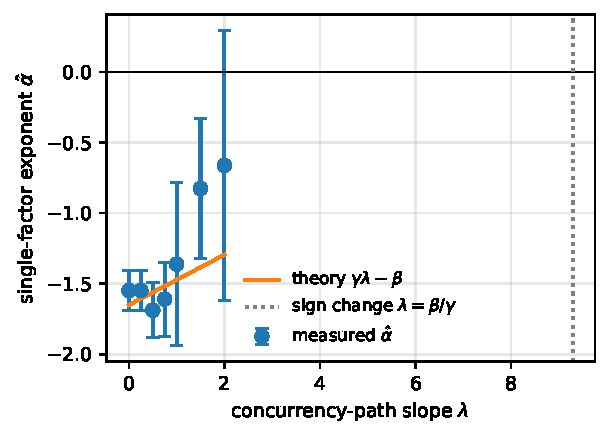
\includegraphics[width=0.75\textwidth]{figures/fig_confounding}
\rule{0.75\textwidth}{0.22\textwidth}
\caption{Measured single-factor exponent $\ahat$ as a function of the
concurrency-path slope $\lambda$, against the theoretical line
$\ghat\lambda-\bhat$. The sign change occurs at $\lambda=\bhat/\ghat$}
\label{fig:confounding}
\end{figure}

The sign of $\ahat$ reverses as $\lambda$ crosses $\bhat/\ghat$, which is the
mechanism of Corollary~\ref{cor:sign}. This provides a direct, measured
explanation for positive single-factor exponents reported in the literature
and in our earlier work~\cite{peniak2026a}, and shows that such exponents
cannot be transferred between testbeds.

\subsection{$\q$-invariance}

Fitting the interaction model~\eqref{eq:ancova} across quotas gives
$\bhat(\q{=}0.20)=\resBetaQlow$, $\bhat(\q{=}0.25)=\resBetaQmid$ and
$\bhat(\q{=}0.33)=\resBetaQhigh$. The partial $F$-test of
$H_{0}:d_{2}=d_{3}=0$ yields $p=\resQinvP$. \TODO{Interpret: if $p$ is large,
Assumption~\ref{as:separable} is not rejected and
Statement~\ref{st:qinvariance} is supported; if small, report the quota range
over which invariance does hold.}

\subsection{Latency sensitivity}

Emulated wide-area latency degrades the consensus exponent from
$\bhat=\resBetaRttZero$ at zero added round-trip time to $\resBetaRttHigh$ at
200~ms. This quantifies how a geographically distributed deployment narrows the
feasibility window of Theorem~\ref{thm:window}.

\subsection{Detector characterization}

Fault-injection runs with ground-truth labels give a detection probability
$\pd=\resPd$, a false-positive rate $\pf=\resPf$, an area under the receiver
operating characteristic of $\resAuc$, and an exchangeable correlation
$\rho=\resRho$ among faulty-validator indicators. These are the inputs
to~\eqref{eq:muB} and~\eqref{eq:pmiss}, and they are measured rather than
assumed as they were in~\cite{peniak2026b}.

\begin{figure}[!t]
\centering
% 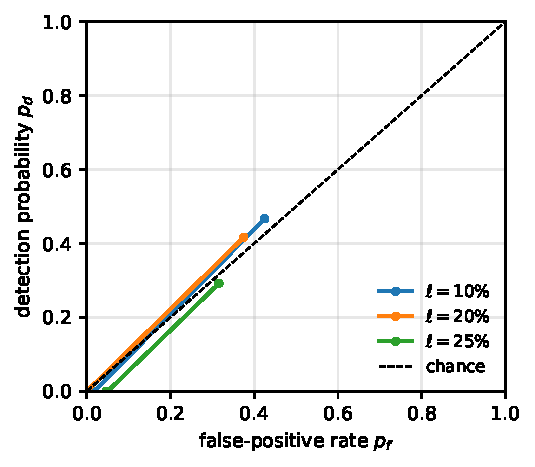
\includegraphics[width=0.7\textwidth]{figures/fig_roc}
\rule{0.7\textwidth}{0.2\textwidth}
\caption{Receiver operating characteristic of the participation detector at
injection levels $\ell\in\{10,20,25\}\%$, with the operating point used in the
sizing study marked}
\label{fig:roc}
\end{figure}

\subsection{Coverage of prediction intervals}

Calibrating on $\n\le9$ and predicting the held-out counts $\resHoldoutN$ gives
empirical coverage $\resCovNinety$ at nominal 90\,\% and $\resCovNinetyFive$ at
nominal 95\,\%. \TODO{State whether the delta-method and bootstrap intervals
agree, and whether coverage is conservative or optimistic.} Reporting coverage
rather than an average percentage error makes the guarantee falsifiable, which
the heuristic accuracy figure of~\cite{peniak2026a} was not.

\subsection{Comparison of scaling models}

Table~\ref{tab:models} compares the bi-factor law against Amdahl's law,
Gustafson's law, the Universal Scalability Law~\eqref{eq:usl} and the
single-factor power law, on held-out data.

\begin{table}[!t]
\caption{Out-of-sample comparison of scaling models on held-out validator
counts}
\label{tab:models}
\centering
\small
\begin{tabular}{lccc}
\headline
Model & Parameters & Held-out log-RMSE & PI coverage at 90\,\% \\
\headline
Linear (no degradation)          & 1 & \TODO{} & \TODO{} \\
Single factor~\cite{peniak2026a} & 2 & \TODO{} & \TODO{} \\
Amdahl~\cite{amdahl1967}         & 2 & \TODO{} & \TODO{} \\
USL~\cite{gunther2007}           & 3 & \TODO{} & \TODO{} \\
Bi-factor (this work)            & 5 & \TODO{} & \resCovNinety \\
\headline
\end{tabular}
\end{table}

\subsection{Sizing ablation}

Applying Algorithm~\ref{alg:sizing} to the workload of Section~\ref{sec:case}
gives $\nmin=\resNminCase$, $\nmax=\resNmaxCase$ and $\nopt=\resNoptCase$.
Table~\ref{tab:ablation} compares the provisioning decision and its cost
against the alternatives.

\begin{table}[!t]
\caption{Sizing decisions and provisioning cost under different scaling models}
\label{tab:ablation}
\centering
\small
\begin{tabular}{lccc}
\headline
Model used for sizing & Recommended $\n$ & Demand met? & Relative cost \\
\headline
Linear extrapolation             & \TODO{} & \TODO{} & \resCostLinear \\
Single factor~\cite{peniak2026a} & \TODO{} & \TODO{} & \resCostSingle \\
USL~\cite{gunther2007}           & \TODO{} & \TODO{} & \resCostUsl \\
Chance-constrained (this work)   & \resNoptCase & yes at $1-\epsp$ & \resCostOurs \\
\headline
\end{tabular}
\end{table}

\subsection{Campaign cost}

The complete campaign comprises \resTotalRuns{} runs consuming
\resCoreHours{} core-hours on the public runner, with a largest measured
validator set of \resNmaxMeasured.
